\section{AUTOMASI PEMBUATAN KNOWLEDGE GRAPH UNTUK PERATURAN
PERUNDANG-UNDANGAN DI
INDONESIA}\label{automasi-pembuatan-knowledge-graph-untuk-peraturan-perundang-undangan-di-indonesia}

\section{BAB 1 PENDAHULUAN}\label{bab-1-pendahuluan}

\subsection{Latar Belakang}\label{latar-belakang}

Peraturan perundang-undangan adalah peraturan tertulis yang memuat norma
hukum yang mengikat secara umum dan dibentuk atau ditetapkan oleh
lembaga negara atau pejabat yang berwenang melalui prosedur yang
ditetapkan dalam peraturan perundang-undangan, sesuai yang dijelaskan
dalam UU Nomor 12 Tahun 2011 Pasal 1 Ayat 2
\href{https://www.pustaka.ut.ac.id/lib/wp-content/uploads/pdfmk/HKUM4403-M1.pdf}{1}.
Peraturan perundang-undangan dapat digunakan untuk menjawab pertanyaan
yang berkaitan dengan hukum, seperti:

\begin{itemize}
\itemsep1pt\parskip0pt\parsep0pt
\item
  Peraturan apa saja yang berlaku pada suatu daerah?
\item
  Apa hubungan suatu peraturan dengan peraturan lain?
\item
  Apa saja peraturan yang mengatur suatu topik?
\end{itemize}

Pertanyaan-pertanyaan tersebut umumnya dapat dijawab oleh seorang ahli
hukum, artinya penerapan peraturan perundang-undangan ini hanya dapat
dilakukan dalam skala kecil dan biaya relatif mahal. Komputer dapat
menjadi alternatif untuk aplikasi tersebut dalam skala lebih besar dan
biaya lebih murah, jika peraturan perundang-undangan berupa data
terstruktur yang dapat diolah oleh komputer. Sayangnya, data peraturan
perundang-undangan umumnya dibuat dalam bentuk data semi-terstruktur,
yaitu berupa dokumen yang memiliki data terstruktur seperti aturan
penomoran dan aturan struktur (seperti bab, pasal, dan ayat), tetapi
penulisan peraturan sendiri dalam bentuk data tidak terstruktur yaitu
teks bahasa manusia.

\begin{figure}[htbp]
\centering

\includegraphics{pictures/terstruktur.png}
\caption{Data Terstruktur dan Tidak Terstruktur dari Dokumen}
\end{figure}

\begin{figure}[htbp]
\centering

\includegraphics{pictures/terstruktur_parsed.svg}
\caption{Hasil Parsing Data Terstruktur dan Tidak Terstruktur dari
Dokumen}
\end{figure}

Gambar diatas merupakan salah satu contoh ekstraksi informasi dari UU
No.11 Tahun 2020 tentang Ketenagakerjaan. Pada gambar diatas, dapat
dilihat bahwa sebagian informasi dapat diekstraksi dari sifat
terstruktur dokumen peraturan perundang-undangan (ditandai dengan warna
merah), dan sebagian informasi lainnya dapat diekstraksi dari data tidak
terstruktur beruba teks (ditandai dengan warna biru). Untuk melakukan
ekstraksi informasi tidak terstruktur seperti pada gambar yaitu ``UU
No.11 Tahun 2020 Pasal 6 menyebut UU No.11 Tahun 2020 Pasal 5 ayat(1)
huruf a'', manusia pertama-tama perlu membaca dari awal kalimat sampai
menemukan pola \emph{string} yang merujuk kepada suatu komponen dokumen
peraturan perundang-undangan, kemudian meng-\emph{infer} informasi
lengkap dari komponen tersebut. Proses konversi \emph{string} ``Pasal 5
ayat (1) huruf a'' menjadi informasi lengkap ``UU No.11 Tahun 2020 Pasal
5 ayat (1) huruf a'' perlu dilakukan secara manual oleh manusia.

Dengan melakukan ekstraksi data dari data tidak terstruktur pada
dokumen, digabung dengan data yang sudah terstruktur, peraturan
perundang-undangan dapat diubah menjadi dapat diolah oleh komputer.
Selain dapat menjawab pertanyaan, representasi \emph{knowledge graph}
juga dapat digunakan untuk analisis karena data sudah terstruktur.
Representasi \emph{knowledge graph} juga memungkinkan untuk dapat
melakukan \emph{reasoning}. Pada skripsi ini, akan dilakukan konversi
dokumen peraturan perundang-undangan menjadi data terstruktur dalam
bentuk \emph{knowledge graph}, dan memberikan contoh pengaplikasian dari
\emph{knowledge graph} peraturan perundang-undangan tersebut.

\begin{figure}[htbp]
\centering

\includegraphics{pictures/outline.svg}
\caption{Outline}
\end{figure}

Beberapa usaha telah dilakukan untuk membuat \emph{vocabulary} untuk
\emph{knowledge graph} peraturan perundang-undangan seperti
\emph{European Legislation Identifier} (ELI)
\href{https://eur-lex.europa.eu/eli-register/about.html}{2}. Tetapi ELI
belum memiliki \emph{vocabulary} untuk struktur dokumen. Sehingga dengan
membuat \emph{vocabulary} yang belum tersedia, diharapkan dapat menjadi
kontribusi dalam mendukung pembuatan \emph{knowledge graph} untuk
dokumen peraturan perundan-undangan.

\subsection{Permasalahan}\label{permasalahan}

Berikut ini adalah rumusan permasalahan dari penelitian yang dilakukan:

\begin{itemize}
\itemsep1pt\parskip0pt\parsep0pt
\item
  Bagaimana cara membuat \emph{legal ontology} untuk memperjelas
  \emph{requirement} dan mempermudah konversi dokumen PDF menjadi
  \emph{knowledge graph}?
\item
  Bagaimana konversi dokumen peraturan perudang-undangan menjadi
  \emph{knowledge graph} dapat dilakukan secara otomatis?
\item
  Apa saja contoh aplikasi dari knowledge graph peraturan
  perundang-undangan tersebut?
\end{itemize}

// TODO: bagaimana melakukan proof of concept untuk yang udah dibuat,
detail untuk maintain, general large scale, evaluasi konversi

\subsection{Batasan Permasalahan}\label{batasan-permasalahan}

// TODO: fokus yang mainteined (UU + non UU), dan coba parsing UU hasil
scraping

\subsection{Sistematika Penulisan}\label{sistematika-penulisan}

\section{BAB 2 TINJAUAN PUSTAKA}\label{bab-2-tinjauan-pustaka}

\subsection{Knowledge Graph}\label{knowledge-graph}

\emph{Knowledge graph} merupakan model data berbasis \emph{graph} yang
menggambarkan entitas dunia nyata dan hubungan antara entitas-entitas
tersebut
\href{https://yashuseth.blog/2019/10/08/introduction-question-answering-knowledge-graphs-kgqa/}{5}.
Sebagai contoh, pada gambar dibawah dapat dilihat terpadat
entitas-entitas yang ditandai dengan bentuk lingkaran, dan hubungan
antara entitas-entitas ditandai dengan bentuk anak panah. Dapat dilihat
pada gambar dibawah bahwa terdapat entitas ``James'' dan ``Louvre'' dan
properti ``has visited'' yang mengarah dari ``James'' ke ``Louvre''.
Relasi tersebut dapat kita anggap sebagai sebuah pengetahuan yang dalam
bahasa manusia dapat dituliskan sebagai ``James pernah mengunjungi
Louvre''. Model data seperti ini cocok untuk menyimpan data dengan
banyak jenis relasi antara entitas seperti pengetahuan umum,
dibandingkan dengan \emph{relational database} yang cocok untuk
menyimpan data dengan relasi antar entitas yang sudah diketahui dan
terbatas.

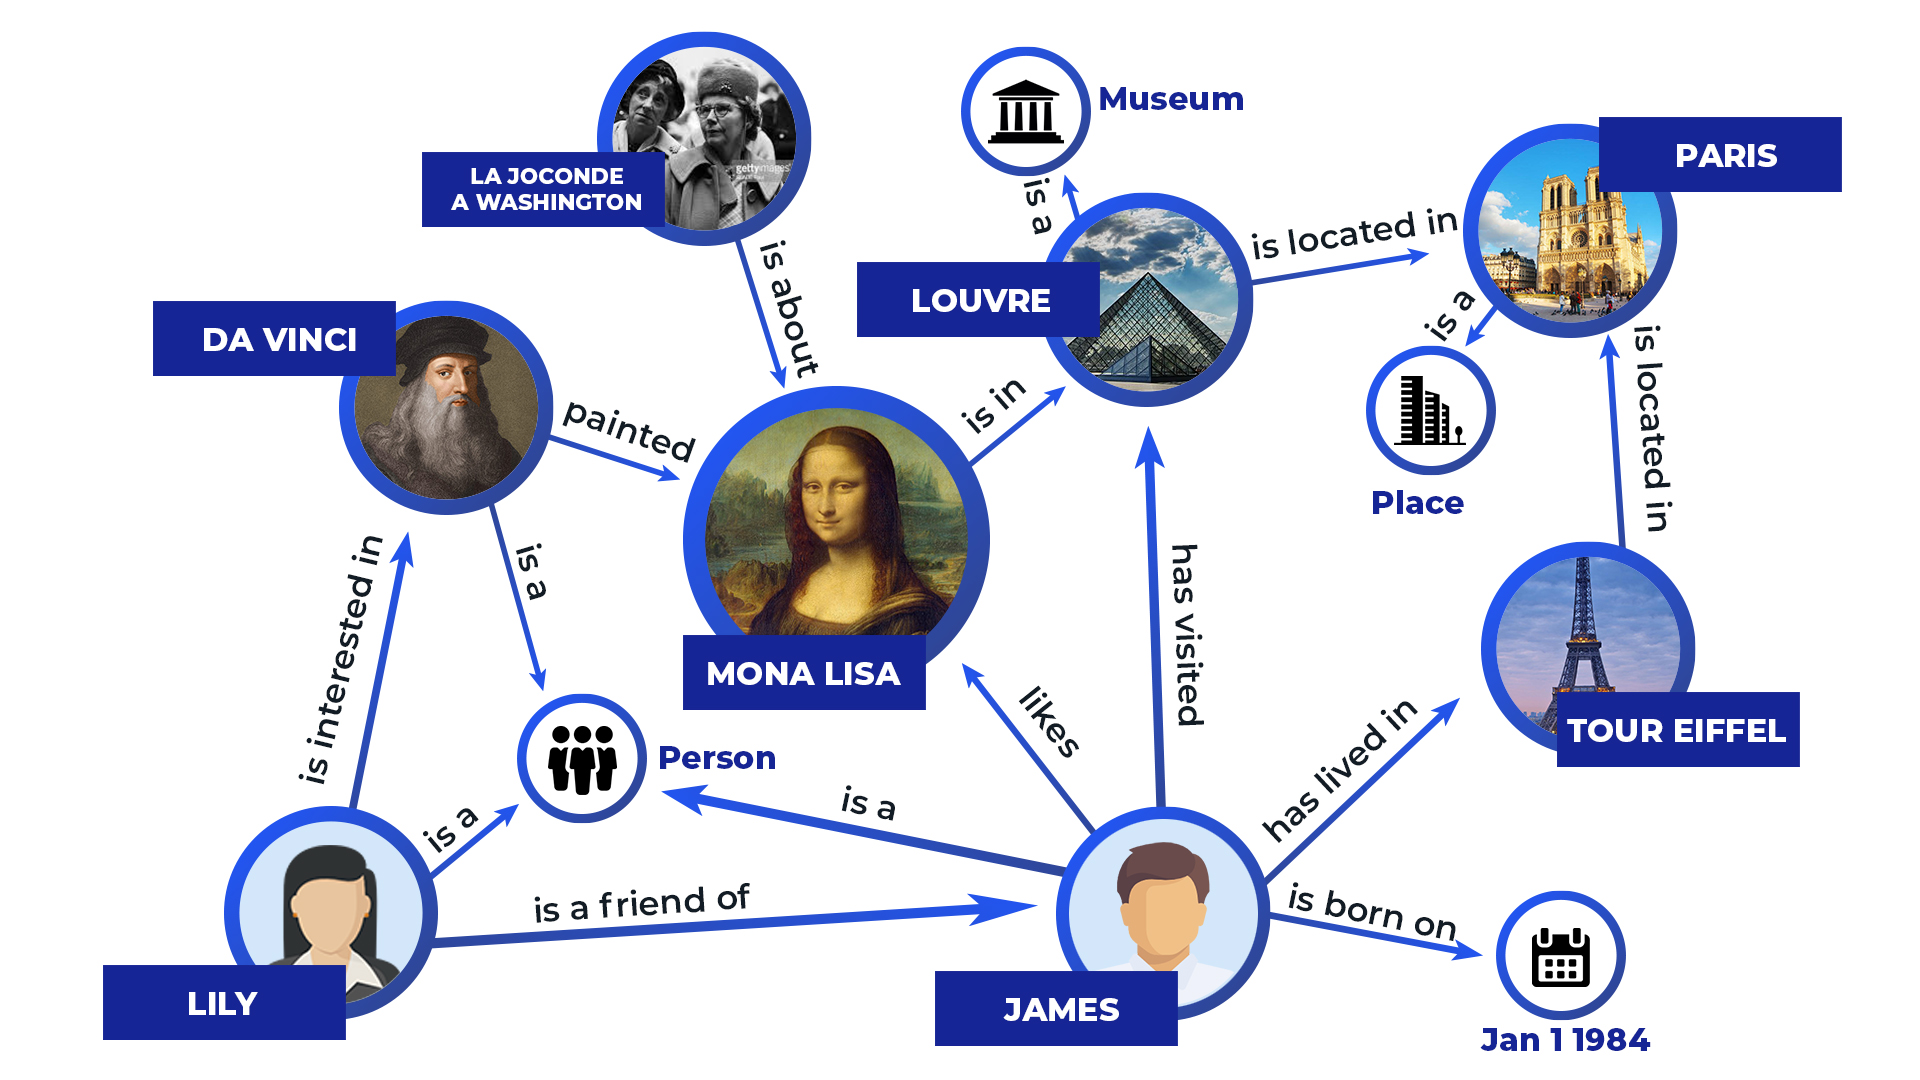
\includegraphics{pictures/knowledge_graph.jpg}
\emph{source}:\url{https://yashuseth.files.wordpress.com/2019/10/knowledge-graph.jpg}

\subsection{Resource Description
Framework}\label{resource-description-framework}

Resource Description Framework (RDF) merupkan model data yang memberikan
pernyataan tentang suatu \emph{resource} dalam bentuk
subjek-properti-objek, atau sering disebut \emph{triple}. Sebuah
\emph{knowledge graph} dapat direpresentasikan sebagai kumpulan
\emph{triple}. Subyek dan properti dalam \emph{triple} direpresentasikan
sebagai Uniform Resource Identifier (URI), sedangkan objek dapat
direpresentasikan dengan URI atau \emph{string literal}. Pada gambar
dibawah, dapat dilihat terdapat \emph{knowledge graph} dengan dua
\emph{triple}. Pada triple 1 subjek, properti, dan objek berturut-turut
adalah
\texttt{https://example.org/james},\texttt{https://example.org/has\_visited},\texttt{https://example.org/louvre}
yang mana semuanya berbentuk URI. Sedangkan pada triple 2 subjek,
properti, dan objek berturut-turut adalah
\texttt{https://example.org/james},\texttt{https://example.org/has\_name},
``james'' . \texttt{https://example.org/james},
\texttt{https://example.org/louvre} berturut-turut merupakan notasi
untuk \emph{resource} entitas James dan Louvre,
\texttt{https://example.org/has\_visited} dan
\texttt{https://example.org/has\_name} merupakan properti yang
menjelaskan hubungan antara subjek dan objek, dan ``james'' adalah
\emph{string literal} yang menunjukan nilai dari nama James.

\begin{figure}[htbp]
\centering

\includegraphics{pictures/triple.svg}
\caption{Triple}
\end{figure}

Terdapat beberapa format berkas dan sintaks untuk mengekspresikan RDF.
Pada penelitian ini, penulis menggunakan format Terse RDF Triple
Language (Turtle). Sebagai contoh, \emph{knowledge graph} diatas dapat
dituliskan dalam format Turtle sebagai berikut.

\begin{verbatim}
<https://example.org/james> <https://example.org/has_visited> <https://example.org/louvre> .
<https://example.org/james> <https://example.org/has_name> "james" .
\end{verbatim}

Dengan fitur format Turtle, dua \emph{triple} diatas dapat ditulis lebih
singkat dengan mengganti prefix URI yang sama menjadi teks yang lebih
singkat, dan menggabungkan penulisan beberapa \emph{triple} dengan
subjek yang sama sehingga subjek hanya perlu dituliskan sekali saja.
Sebagai contoh, karena sebagaian besar URI memiliki prefix
\texttt{https://example.org/}, kita dapat menggantinya dengan
\emph{string} \texttt{ex} dengan mendeklarasikan
\texttt{@prefix ex: \textless{}https://example.org/\textgreater{} .}.
Kedua \emph{triple} juga memiliki subjek yang sama yaitu
\texttt{https://example.org/james}, oleh karena itu, penulisan kedua
turtle bisa digabung dengan hanya menuliskan subjek sebanyak satu kali,
kemudian menuliskan properti dan objek dipisah dengan tanda titik koma .
Berikut adalah contoh penulisan dua \emph{triple} diatas dalam bentuk
yang lebih singkat dan lebih mudah dibaca oleh manusia.

\begin{verbatim}
@prefix ex: <https://example.org/> .

ex:james 
  ex:has_visited ex:louvre ;
  ex:has_name "james" .
\end{verbatim}

\subsection{SPARQL}\label{sparql}

SPARQL merupakan salahsatu RDF \emph{query language} yaitu bahasa yang
mampu mengambil atau mengubah data yang disimpan dalam format RDF.
Sintaks SPARQL memiliki beberapa kesamaan dengan SQL, contohnya sebuah
variabel diawali dengan tanda tanya seperti \texttt{?name}. Berikut
adalah penjelasan sintaks SPARQL.

\begin{itemize}
\itemsep1pt\parskip0pt\parsep0pt
\item
  \texttt{PREFIX}: Mendeklarasikan pemetaan prefix URI menjadi
  \emph{string} yang lebih singkat. Hal ini dilakukan agar \emph{query}
  lebih mudah dibaca oleh manusia seperti sintaks \texttt{@prefix} pada
  Turtle.
\item
  \texttt{SELECT}: Menyatakan variabel yang akan ditampilkan sebagai
  output dari \emph{query}.
\item
  \texttt{WHERE}: Menyatakan kondisi \emph{triple} yang akan ditampilkan
  pada output.
\end{itemize}

Berikut adalah contoh-contoh \emph{query} SPARQL yang dilakukan pada
contoh \emph{knowledge graph} pada subbab sebelumnya.

\subsubsection{Contoh Query 1}\label{contoh-query-1}

\emph{Query} ini bertujuan untuk menampilkan semua \emph{triple} yang
terdapat pada \emph{knowledge graph}.

\begin{verbatim}
PREFIX ex: <https://example.org/>
SELECT ?s 
       ?p
       ?o
WHERE
  {
    ?s ?p ?o
  }
\end{verbatim}

Output dari \emph{query} tersebut adalah sebagai berikut.

\begin{longtable}[c]{@{}lll@{}}
\toprule\addlinespace
?s & ?p & ?o
\\\addlinespace
\midrule\endhead
ex:james & ex:has\_visited & ex:louvre
\\\addlinespace
ex:james & ex:has\_name & ``james''
\\\addlinespace
\bottomrule
\end{longtable}

\subsubsection{Contoh Query 2}\label{contoh-query-2}

\emph{Query} ini bertujuan untuk menampilkan semua properti dan objek
pada \emph{triple} dengan subjek \texttt{https://example.org/james}.

\begin{verbatim}
PREFIX ex: <https://example.org/>
SELECT ?p
       ?o
WHERE
  {
    ex:james ?p ?o
  }
\end{verbatim}

Output dari \emph{query} tersebut adalah sebagai berikut.

\begin{longtable}[c]{@{}ll@{}}
\toprule\addlinespace
?p & ?o
\\\addlinespace
\midrule\endhead
ex:has\_visited & ex:louvre
\\\addlinespace
ex:has\_name & ``james''
\\\addlinespace
\bottomrule
\end{longtable}

\subsubsection{Contoh Query 3}\label{contoh-query-3}

\emph{Query} ini bertujuan untuk menampilkan semua objek pada
\emph{triple} dengan subjek \texttt{https://example.org/james} dan
properti \texttt{https://example.org/has\_visited}. Artinya,
\emph{query} ini menampilkan semua tempat yang pernah dikunjungi james.

\begin{verbatim}
PREFIX ex: <https://example.org/>
SELECT ?visited_place
WHERE
  {
    ex:james ex:has_visited ?visited_place
  }
\end{verbatim}

Output dari \emph{query} tersebut adalah sebagai berikut.

\textbar{} ?visited\_place \textbar{}
\textbar{}----------------\textbar{} \textbar{} ex:louvre \textbar{}

\subsection{Peraturan
Perundang-undangan}\label{peraturan-perundang-undangan}

??? boleh ngequote sebanyak apa?

Menurut Undang-Undang Nomor 10 Tahun 2004 Pasal 7 Ayat 1, peraturan
perundang-undangan adalah peraturan tertulis yang dibentuk oleh lembaga
negara atau pejabat yang berwenang dan mengikat secara umum. Jenis dan
hierarki peraturan perundang-undangan terdiri atas:

\begin{itemize}
\itemsep1pt\parskip0pt\parsep0pt
\item
  Undang-Undang Dasar Negara Republik Indonesia Tahun 1945
\item
  Undang-Undang/Peraturan Pemerintah Pengganti Undang-Undang
\item
  Peraturan Pemerintah
\item
  Peraturan Presiden
\item
  Peraturan Daerah
\end{itemize}

Berikut adalah beberapa peranan perundang-undangan untuk Indonesia
\href{https://www.pustaka.ut.ac.id/lib/wp-content/uploads/pdfmk/HKUM4403-M1.pdf}{1}:

\begin{itemize}
\itemsep1pt\parskip0pt\parsep0pt
\item
  Peraturan perundang-undangan merupakan kaidah hukum yang mudah dikenal
  (diidentifikasi), mudah diketemukan kembali, dan mudah ditelusuri.
  Sebagai kaidah hukum tertulis, bentuk, jenis,dan tempatnya jelas.
  Begitu pula pembuatnya.
\item
  Peraturan perundang-undangan memberikan kepastian hukum yang lebih
  nyata karena kaidah-kaidahnya mudah diidentifikasi dan mudah
  diketemukan kembali.
\item
  Struktur dan sistematika peraturan perundang-undangan lebih jelas
  sehingga memungkinkan untuk diperiksa kembali dan diuji baik segi-segi
  formal maupun materi muatannya.
\item
  Pembentukan dan pengembangan peraturan perundang-undangan dapat
  direncanakan. Faktor ini sangat penting bagi negara-negara yang sedang
  membangun termasuk membangun sistem hukum baru yang sesuai dengan
  kebutuhan dan perkembangan masyarakat.
\end{itemize}

Menurut lampiran Undang-Undang Nomor 10 Tahun 2004, struktur peraturan
perundang--undangan terdiri atas:

\begin{itemize}
\itemsep1pt\parskip0pt\parsep0pt
\item
  Judul
\item
  Pembukaan
\item
  Batang Tubuh
\item
  Penutup
\item
  Penjelasan (jika diperlukan)
\item
  Lampiran (jika diperlukan)
\end{itemize}

Bagian judul, pembukaan, dan penutup memuat metadata dari peraturan
perundang-undangan tersebut seperti jenis, nomor, tahun pengundangan
atau penetapan, nama, jabatan pembentuk, konsiderans, kasar Hukum,
peraturan perundang-undangan. Konsiderans memuat uraian singkat mengenai
pokok--pokok pikiran yang menjadi latar belakang dan alasan pembuatan
peraturan perundang--undangan. Dasar Hukum memuat dasar kewenangan
pembuatan peraturan perundang-undangan dan peraturan perundang--undangan
yang memerintahkan pembuatan peraturan perundang--undangan tersebut.
Oleh karena itu, kita dapat melihat keterkaitan antara peraturan
perundang-undangan dengan melihat konsiderans dan dasar hukum dari
peraturan tersebut.

Batang tubuh peraturan perundang-undangan memuat semua substansi
peraturan perundang-undangan yang dirumuskan dalam pasal. Pengelompokkan
materi peraturan perundang-undangan dapat disusun secara sistematis
dalam buku, bab, bagian, dan paragraf atas dasar kesamaan materi. Pasal
dapat dirinci ke dalam beberapa ayat. Pasal dan ayat dapat dibuat dalam
bentuk kalimat maupun tabulasi rincian. Dalam bentuk tabulasi rincian,
setiap rincian harus dapat dibaca sebagai satu rangkaian kesatuan dengan
frase pembuka dan setiap rincian diawali dengan huruf (abjad) kecil dan
diberi tanda baca titik. Suatu rincian dapat dibagi lagi ke unsur
rincian yang lebih kecil.

Saat ini pembuatan dan pemanfaatan peraturan perundang-undangan masih
dilakukan secara manual oleh manusia. Pembuatan peraturan
perundang-undangan dilakukan dengan mengetikkan konten peraturan
tersebut dengan format yang telah ditentukan. Metode pembuatan tersebut
tidak masalah jika hanya akan dibaca oleh manusia karena manusia secara
tidak sadar dapat melihat hirarki visual dari dokumen tersebut dan
membuat data yang dilihatnya terstruktur di dalam otak. Metode ini
membuat pemanfaatan peraturan perundang-undangan oleh mesin menjadi
kurang efisien karena mesin perlu melakukan proses tambahan yaitu
mengkonversi gambar menjadi data terstruktur.

\subsection{Pemodelan European Legislation Identifier
(ELI)}\label{pemodelan-european-legislation-identifier-eli}

ELI merupakan sistem untuk membuat peraturan perundang-undangan tersedia
secara daring dalam format terstandardisasi, sehingga dapat diakses dan
digunakan oleh berbagai instansi. ELI bertujuan untuk untuk
memfasilitasi akses, berbagi dan interkoneksi informasi hukum yang
diterbitkan melalui nasional, Eropa dan sistem informasi hukum global
{[}6{]}. ELI dibangun berdasarkan persetujuan antara negara-negara EU.
Spesifikasi yang terdapat pada ELI antara lain:

\begin{itemize}
\itemsep1pt\parskip0pt\parsep0pt
\item
  URI untuk informasi peraturan perundang-undangan.
\item
  Metadata yang mendeskripsikan informasi peraturan perundang-undangan.
\end{itemize}

// TODO: terlalu singkat, ksh konsepnya gmn dan contoh pemodelan ELI utk
suatu peraturan

// TODO: ELI jg msh simpel. Bs dijelaskan motivasi ELI, serta apa contoh
konsep2 yg sdh ada di ELI ontology, serta yg belum ada.

// TODO: - ELI kekurangan lainnya ya lbh condong ke pemodelan peraturan
di Eropa, bukan di Indonesia. Misal, gak ada namanya Peraturan
Pemerintah, atau Pergub di ELI :)

\section{BAB 3 METODOLOGI}\label{bab-3-metodologi}

// TODO: Maintained docs masukin sini

// TODO: Utk yg metodologi, sbnrnya standar aja, dimulai dari pertanyaan
riset, lalu pengembangan ontology (URI scheming masuk ke pengembagan
ontology), pengembangan sistem konversi, baru lalu use case evaluation
(ini yg legal KG advanced querying, legal KG chatbot, legal KG
visualization) baru large scale eval (ini yg coba konversi peraturan dlm
jumlah besar dan kita sampling utk evaluasi correctnessnya)

TODO: suatu KG construction dimulai dengan competency questions
(requirements). Saran sy: coba baca serta rangkum (di Bab 2) dan
terapkan ini:
www.ksl.stanford.edu/people/dlm/papers/ontology-tutorial-noy-mcguinness-abstract.html
???

\section{BAB 4 RANCANGAN}\label{bab-4-rancangan}

\subsection{Perancangan URI}\label{perancangan-uri}

Setiap entitas yang berbeda perlu diberikan URI yang berbeda.
Penggabungan KG sangat umum dilakukan karena secara struktur dapat
dilakukan dengan mudah, dan dapat memperkuat data dari masing-masing KG.
KG memiliki entitas-entitas dengan URI yang unik, oleh karena itu saat
menggabungkan sebuah KG A dan sebuah KG B, entitas yang berbeda harus
memiliki URI yang berbeda. Sebuah masalah dapat terjadi apabila URI
tidak dirancang dengan benar. Sebagai contoh, apabila terdapat entitas
dari KG A dengan URI \texttt{http://example.org/trump} dengan maksud
Donald Trump mantan presiden Amerika Serikat, dan entitas dari KG B
dengan URI yang sama dengan maksud permainan kartu Trump, saat kedua KG
ini digabung akan menjadi informasi yang berkontradiksi.

Pada penelitian ini, semua URI menggunakan prefix
\texttt{http://example.org/legal/} yang selanjutnya akan disebut
\emph{basePrefix}. Prefix ini dapat diganti dalam program agar dapat
disesuaikan oleh pengguna program. Semua entitas dokumen dan komponennya
menggunakan prefix URI \texttt{http://example.org/legal/peraturan} yang
selanjutnya disebut \emph{peraturanPrefix}, dan semua resource lainnya
menggunakan \texttt{http://example.org/legal/ontology} yang selanjutnya
disebut \emph{ontoPrefix}.

\subsection{Perancangan URI Class}\label{perancangan-uri-class}

URI Class adalah URI yang menjelaskan \emph{class} dari entitas
tersebut. Semua URI Class mengikuti pola
\texttt{\{ontoPrefix\}/\{className\}} dimana \texttt{className} adalah
nama \emph{class} tersebut. Berikut adalah semua \emph{class} komponen
beserta URI dan deskripsinya.

\begin{longtable}[c]{@{}ll@{}}
\toprule\addlinespace
Nama Class & Deskripsi
\\\addlinespace
\midrule\endhead
\texttt{Peraturan} & Peraturan perundang-undangan
\\\addlinespace
\texttt{DaftarBab} & Daftar satu atau lebih bab
\\\addlinespace
\texttt{Bab} & Bab
\\\addlinespace
\texttt{DaftarBagian} & Daftar satu atau lebih bagian
\\\addlinespace
\texttt{Bagian} & Bagian
\\\addlinespace
\texttt{DaftarParagraf} & Daftar satu atau lebih paragraf
\\\addlinespace
\texttt{Paragraf} & Paragraf
\\\addlinespace
\texttt{DaftarPasal} & Daftar satu atau lebih pasal
\\\addlinespace
\texttt{Pasal} & Pasal
\\\addlinespace
\texttt{VersiPasal} & Versi dari sebuah pasal. Sebuah pasal dapat
memiliki satu atau lebih versi dari hasil amandemen
\\\addlinespace
\texttt{DaftarAyat} & Daftar satu atau lebih ayat
\\\addlinespace
\texttt{Ayat} & Ayat
\\\addlinespace
\texttt{DaftarHuruf} & Daftar satu atau lebih huruf atau nomor
\\\addlinespace
\texttt{Huruf} & Huruf atau nomor
\\\addlinespace
\texttt{Menimbang} & Hal yang ditimbang oleh suatu peraturan
\\\addlinespace
\texttt{Mengingat} & Hal yang diingat oleh suatu peraturan
\\\addlinespace
\texttt{Segmen} & Segmen teks. Dapat memiliki rujukan ke suatu komponen
peraturan
\\\addlinespace
\bottomrule
\end{longtable}

\subsection{Perancangan URI Komponen Peraturan
Perundang-undangan}\label{perancangan-uri-komponen-peraturan-perundang-undangan}

URI peraturan perundang-undangan diawali oleh \emph{peraturanPrefix},
kemudian diikuti oleh string yang mengidentifikasi peraturan tersebut.
URI peraturan ini akan digunakan oleh entitas sebagai prefix yang
selanjutnya akan disebut \emph{docURI}. Berikut adalah jenis peraturan
perundang-undangan yang diimplementasi pada penelitian ini beserta pola
URI nya. Variabel akan dikurung dengan kurung kurawal \texttt{\{\}}.

\begin{longtable}[c]{@{}lll@{}}
\toprule\addlinespace
Jenis Peraturan & Pola URI & Penjelasan variabel
\\\addlinespace
\midrule\endhead
Undang-Undang Dasar 1945 & \texttt{\{peraturanPrefix\}/uud} &
\\\addlinespace
Undang-Undang & \texttt{\{peraturanPrefix\}/uu/\{tahun\}/\{nomor\}} &
\texttt{tahun}: tahun peraturan
\\\addlinespace
& & \texttt{nomor}: nomor peraturan
\\\addlinespace
Peraturan Pemerintah &
\texttt{\{peraturanPrefix\}/pp/\{tahun\}/\{nomor\}} & \texttt{tahun}:
tahun peraturan
\\\addlinespace
& & \texttt{nomor}: nomor peraturan
\\\addlinespace
Peraturan Daerah Provinsi DKI Jakarta &
\texttt{\{peraturanPrefix\}/perda\_provinsi\_dki\_jakarta/\{tahun\}/\{nomor\}}
& \texttt{tahun}: tahun peraturan
\\\addlinespace
& & \texttt{nomor}: nomor peraturan
\\\addlinespace
Peraturan Gubernur DKI Jakarta &
\texttt{\{peraturanPrefix\}/pergub\_dki\_jakarta/\{tahun\}/\{nomor\}} &
\texttt{tahun}: tahun peraturan
\\\addlinespace
& & \texttt{nomor}: nomor peraturan
\\\addlinespace
Peraturan Walikota Malang &
\texttt{\{peraturanPrefix\}/perwali\_malang/\{tahun\}/\{nomor\}} &
\texttt{tahun}: tahun peraturan
\\\addlinespace
& & \texttt{nomor}: nomor peraturan
\\\addlinespace
\bottomrule
\end{longtable}

Setiap komponen dokumen merupakan entitas, dan memiliki URI. URI sebuah
komponen didahului oleh \emph{docURI} dan semua komponen yang
mengatasinya. Berikut adalah jenis komponen peraturan perundang-undangan
beserta pola URI nya.

\begin{longtable}[c]{@{}lll@{}}
\toprule\addlinespace
Class Komponen & Pola URI & Penjelasan variabel
\\\addlinespace
\midrule\endhead
\texttt{DaftarBab} & \texttt{\{docURI\}/bab} & \texttt{docURI}: URI
peraturan yang mengatasi
\\\addlinespace
\texttt{Bab} & \texttt{\{daftarBabURI\}/\{no\}} & \texttt{daftarBabURI}:
URI \texttt{DaftarBab} yang mengatasi
\\\addlinespace
& & \texttt{no}: Nomor bab
\\\addlinespace
\texttt{DaftarBagian} & \texttt{\{babURI\}/bagian} & \texttt{babURI}:
URI \texttt{Bab} yang mengatasi
\\\addlinespace
\texttt{Bagian} & \texttt{\{daftarBagianURI\}/\{no\}} &
\texttt{daftarBagianURI}: URI \texttt{DaftarBagian} yang mengatasi
\\\addlinespace
& & \texttt{no}: Nomor bagian
\\\addlinespace
\texttt{DaftarParagraf} & \texttt{\{bagianURI\}/paragraf} &
\texttt{bagianURI}: URI \texttt{Bagian} yang mengatasi
\\\addlinespace
\texttt{Paragraf} & \texttt{\{daftarParagrafURI\}/\{no\}} &
\texttt{daftarParagrafURI}: URI \texttt{DaftarBagian} yang mengatasi
\\\addlinespace
& & \texttt{no}: Nomor paragraf
\\\addlinespace
\texttt{DaftarPasal} & \texttt{\{parentURI\}/daftarpasal} &
\texttt{parentURI}: URI \texttt{Bab}, \texttt{Bagian}, \texttt{Paragraf}
yang mengatasi
\\\addlinespace
\texttt{Pasal} & \texttt{\{docURI\}/pasal/\{no\}} & \texttt{docURI}: URI
peraturan yang mengatasi
\\\addlinespace
& & \texttt{no}: Nomor pasal
\\\addlinespace
\texttt{VersiPasal} & \texttt{\{pasalURI\}/versi/\{date\}} &
\texttt{pasalURI}: URI \texttt{Pasal} yang mengatasi
\\\addlinespace
& & \texttt{date}: Tanggal disahkan
\\\addlinespace
\texttt{DaftarAyat} & \texttt{\{pasalURI\}/ayat} & \texttt{pasalURI}:
URI \texttt{Pasal} yang mengatasi
\\\addlinespace
\texttt{Ayat} & \texttt{\{daftarAyatURI\}/\{no\}} &
\texttt{daftarAyatURI}: URI \texttt{DaftarAyat} yang mengatasi
\\\addlinespace
& & \texttt{no}: Nomor ayat
\\\addlinespace
\texttt{DaftarHuruf} & \texttt{\{parentURI\}/huruf} &
\texttt{parentURI}: URI \texttt{Ayat}, \texttt{Huruf},
\texttt{VersiPasal}, \texttt{Menimbang}, \texttt{Mengingat}, yang
mengatasi
\\\addlinespace
\texttt{Huruf} & \texttt{\{daftarHurufURI\}/\{id\}} &
\texttt{daftarHurufURI}: URI \texttt{DaftarHuruf} yang mengatasi
\\\addlinespace
& & \texttt{id}: Nomor atau huruf
\\\addlinespace
\texttt{Menimbang} & \texttt{\{docURI\}/menimbang} & \texttt{docURI}:
URI peraturan yang mengatasi
\\\addlinespace
\texttt{Mengingat} & \texttt{\{docURI\}/mengingat} & \texttt{docURI}:
URI peraturan yang mengatasi
\\\addlinespace
\texttt{Segmen} & \texttt{\{parentURI\}/\{name\}} & \texttt{parentURI}:
URI \texttt{Ayat}, \texttt{Huruf}, \texttt{DaftarHuruf},
\texttt{VersiPasal}, \texttt{Menimbang}, \texttt{Mengingat}, yang
mengatasi
\\\addlinespace
& & \texttt{name}: Nama teks
\\\addlinespace
\bottomrule
\end{longtable}

\subsection{Perancangan URI Properti}\label{perancangan-uri-properti}

Properti ditandai dengan URI yang memiliki pola
\texttt{\{ontoPrefix\}/\{name\}} dimana \texttt{name} adalah nama dari
properti tersebut. Properti menghubungkan subjek dan objek. Subjek
adalah berupa URI komponen, sedangkan objek dapat berupa URI komponen,
string, \emph{number} (bilangan), atau \emph{date} (tanggal).

\begin{longtable}[c]{@{}llll@{}}
\toprule\addlinespace
Nama Properti & Subjek & Objek & Deskripsi
\\\addlinespace
\midrule\endhead
\texttt{nomor} & \texttt{Bab}, \texttt{Bagian}, \texttt{Paragraf},
\texttt{Pasal}, \texttt{Ayat}, \texttt{Huruf} & string, number & Nomor
atau huruf \emph{identifier} dari komponen
\\\addlinespace
\texttt{teks} & \texttt{Ayat}, \texttt{VersiPasal}, \texttt{Segmen} &
string & teks dari komponen
\\\addlinespace
\texttt{bab} & \texttt{DaftarBab} & \texttt{Bab} & Bab
\\\addlinespace
\texttt{bagian} & \texttt{DaftarBagian} & \texttt{Bagian} & Bagian
\\\addlinespace
\texttt{paragraf} & \texttt{DaftarParagraf} & \texttt{Paragraf} &
Paragraf
\\\addlinespace
\texttt{pasal} & \texttt{DaftarPasal} & \texttt{Pasal} & Pasal
\\\addlinespace
\texttt{ayat} & \texttt{DaftarAyat} & \texttt{Ayat} & Ayat
\\\addlinespace
\texttt{huruf} & \texttt{DaftarHuruf} & \texttt{Huruf} & Huruf
\\\addlinespace
\texttt{segmen} & \texttt{Mengigat},\texttt{Menimbang},
\texttt{Paragraf}, \texttt{VersiPasal}, \texttt{Huruf},
\texttt{DaftarHuruf} & \texttt{Segmen} & Segmen
\\\addlinespace
\texttt{daftarBab} & \texttt{Peraturan} & \texttt{DaftarBab} & DaftarBab
\\\addlinespace
\texttt{daftarBagian} & \texttt{Bab} & \texttt{Daftarbagian} &
DaftarBagian
\\\addlinespace
\texttt{daftarParagraf} & \texttt{Bagian} & \texttt{DaftarParagraf} &
DaftarParagraf
\\\addlinespace
\texttt{daftarPasal} & \texttt{Peraturan},\texttt{Bab},
\texttt{Paragraf}, \texttt{Bagian} & \texttt{DaftarPasal} & DaftarPasal
\\\addlinespace
\texttt{daftarAyat} & \texttt{Pasal} & \texttt{DaftarAyat} & DaftarAyat
\\\addlinespace
\texttt{daftarHuruf} &
\texttt{VersiPasal},\texttt{Ayat},\texttt{Huruf},\texttt{Menimbang},\texttt{Mengingat}
& \texttt{DaftarHuruf} & DaftarHuruf
\\\addlinespace
\texttt{merujuk} & \texttt{Segmen} & entitas apapun & Teks merujuk suatu
entitas
\\\addlinespace
\texttt{mengubah} & \texttt{Huruf} & \texttt{VersiPasal} & Pengubahan
pasal
\\\addlinespace
\texttt{menghapus} & \texttt{Huruf} & \texttt{VersiPasal} & Penghapusan
pasal
\\\addlinespace
\texttt{menyisipkan} & \texttt{Huruf} & \texttt{VersiPasal} & Penyisipan
pasal
\\\addlinespace
\texttt{tanggal} & \texttt{VersiPasal} & date & Tanggal
\\\addlinespace
\texttt{jenisVersi} & \texttt{VersiPasal} & `orisinal', `penyisipan',
`pengubahan', `penghapusan' & Jenis versi
\\\addlinespace
\texttt{versi} & \texttt{Pasal} & \texttt{VersiPasal} & Versi suatu
komponen
\\\addlinespace
\texttt{tentang} & \texttt{Peraturan} & string & Peraturan tentang
\\\addlinespace
\texttt{menimbang} & \texttt{Peraturan} & \texttt{Menimbang} & Peraturan
menimbang
\\\addlinespace
\texttt{mengingat} & \texttt{Peraturan} & \texttt{Mengingat} & Peraturan
mengingat
\\\addlinespace
\texttt{disahkanPada} & \texttt{Peraturan} & date & Peraturan disahkan
pada tanggal
\\\addlinespace
\texttt{disahkanDi} & \texttt{Peraturan} & string & Peraturan disahkan
di lokasi
\\\addlinespace
\texttt{disahkanOleh} & \texttt{Peraturan} & string & Peraturan disahkan
oleh
\\\addlinespace
\texttt{jabatanPengesah} & \texttt{Peraturan} & string & Jabatan
pengesah peraturan
\\\addlinespace
\texttt{bagianDari} & komponen apapun & komponen apapun & Komponen
subjek adalah bagian dari komponen objek
\\\addlinespace
\bottomrule
\end{longtable}

\section{BAB 5 IMPLEMENTASI}\label{bab-5-implementasi}

\subsection{OCR Ulang Berkas PDF}\label{ocr-ulang-berkas-pdf}

Dokumen peraturan perundang-undangan yang digunakan pada penelitian
didapatkan dalam format berkas PDF. Penulis pada awalnya mencoba
langsung mengekstraksi data dari PDF, tetapi penulis menemukan
kesulitan. Salahsatu kesulitan yang penulis temui adalah terdapatnya
salah pemindaian pada berkas PDF. Sebagai contoh, terdapat teks yang
tertulis \texttt{Pasal} tetapi mengandung data \texttt{Pasai}. Selain
itu, penulis juga menemukan bahwa setiap dokumen mengandung keslahan
pemindaian yang bervariasi. Untuk suatu kasus, teks \texttt{(2)} selalu
terdeteksi sebagai \texttt{(21} pada suatu dokumen, tetapi tidak pada
dokumen lainnya. Pada kasus lainnya terdapat dokumen yang hampir tidak
memiliki kesalahan pemindaian dan juga terdapat dokumen yang teksnya
tidak dapat dibaca samasekali.

Walaupun dokumen-dokumen tersebut dipelihara oleh satu lembaga pada satu
situs web, yaitu oleh Dewan Perwakilan Rakyat pada situs web
dpr.go.id/jdih, masing-masing dokumen dibuat kedalam berkas PDF dengan
cara yang berbeda-beda. Penulis tidak dapat mengetahui secara pasti
metode apa yang digunakan, tetapi dari metadata yang didapatkan dari
berkas PDF, penulis dapat membuat beberapa dugaan. Pada berkas PDF,
terdapat metadata dengan nama \textbf{Creator}, dimana pada
dokumen-dokumen peraturan Perudang-udangan yang didapatkan, tercantum
nama-nama alat pencetak atau merk dari pencetak tersebut. Dari informasi
tersebut penulis menduga bahwa terdapat sebagian peraturan
perundang-undangan yang dibuat menjadi PDF dengan mencetaknya menjadi
kertas terlebih dahulu kemudian di pindai oleh pemindai dan sebagian
lainnya dikonversi langsung dari berkas \emph{.docx}. Data yang dipindai
adalah berupa gambar, artinya teks yang terdapat pada berkas PDF adalah
hasil OCR (\emph{optical character recognition}) oleh pemindai tersebut.
Berikut adalah salahsatu contoh dokumen beserta data yang tercantum
sebagai \textbf{Creator} dan contoh kesalahan pemindaiannya yang banyak
terjadi.

\begin{longtable}[c]{@{}lll@{}}
\toprule\addlinespace
Dokumen & \textbf{Creator} & Kesalahan pemindaian
\\\addlinespace
\midrule\endhead
UU Nomor 13 Tahun 2003 & ScanSoft PDF Create! 4 & - (tidak ada)
\\\addlinespace
UU Nomor 6 Tahun 2018 & Canon & \texttt{(2)} selalu dipindai
\texttt{(21}
\\\addlinespace
PP Nomor 34 Tahun 2021 & Fuji Xerox B9100 & data teks tidak terbaca
\\\addlinespace
\bottomrule
\end{longtable}

Pemindaian berkas PDF dengan metode yang berbeda-beda memberikan
kualitas hasil pemindaian yang berbeda-beda dan kesalahan pemindaian
yang tidak konsisten. Untuk menyelesaikan masalah ini, penulis melakukan
OCR ulang terhadap semua dokumen yang akan di konversi. Dengan melakukan
OCR ulang menggunakan satu metode yang sama, penulis tidak hanya
berhasil mendapatkan data hasil pemindaian berkas PDF dengan kualitas
pemindaian yang konsisten untuk semua dokumen. Penulis memilih
menggunakan Tesseract OCR
\href{https://github.com/tesseract-ocr/tesseract}{4} sebagai metode OCR
karena sifatnya \emph{open source} dan mendukung Bahasa Indonesia
sebagai bahasa yang dipindai.

Untuk melakukan OCR ulang perlu dilakukan instalasi program yang
dibutuhkan yang dapat dilakukan dengan \emph{command} berikut pada
sistem operasi Ubuntu 20.04. \texttt{ocrmypdf} merupakan \emph{wrapper}
untuk Tesseract OCR dan \texttt{tesseract-ocr-ind} adalah program
tambahan untuk dapat melakukan OCR menjadi teks Bahasa Indonesia.

\begin{Shaded}
\begin{Highlighting}[]
\KeywordTok{sudo} \NormalTok{apt update}
\KeywordTok{sudo} \NormalTok{apt install ocrmypdf tesseract-ocr-ind -y}
\end{Highlighting}
\end{Shaded}

Setelah program diinstall, OCR dapat dilakukan dengan menjalankan
\emph{command} dibawah. Pada contoh dibawah dilakukan konversi
\texttt{UU-2021-34.pdf} yang sudah ada menjadi
\texttt{UU-2021-34\_OCR.pdf} hasil OCR. Opsi \texttt{-{}-force-ocr}
diperlukan untuk melakukan OCR ulang pada berkas PDF yang sudah memiliki
teks hasil OCR untuk di \emph{overwrite}. Opsi \texttt{-{}-jobs 4}
menjalankan \emph{command} dengan 4 \emph{core} CPU, bilangan pada opsi
ini dapat diganti sesuai kebutuhan. Opsi
\texttt{-{}-tesseract-config tesseract-config.cfg} menjalankan
\emph{command} dengan konfigurasi yang diberikan.

\begin{Shaded}
\begin{Highlighting}[]
\KeywordTok{ocrmypdf} \NormalTok{-l ind --force-ocr --jobs 4 --tesseract-config tesseract-config.cfg UU-2021-34.pdf UU-2021-34_OCR.pdf}
\end{Highlighting}
\end{Shaded}

Konfigurasi Tesseract OCR yang digunakan adalah
\texttt{tessedit\_pageseg\_mode 4} seperti yang terlihat pada isi file
konfigurasi dibawah. \texttt{tessedit\_pageseg\_mode 4} digunakan agar
Tesseract OCR mendeteksi teks sebagai \emph{block}, bukan \emph{word}
atau \emph{character}.

\begin{verbatim}
# tesseract-config.cfg
tessedit_pageseg_mode 4
\end{verbatim}

\subsection{Ekstraksi Berkas PDF menjadi Data
\emph{Span}}\label{ekstraksi-berkas-pdf-menjadi-data-span}

\subsubsection{Data \emph{Span}}\label{data-span}

Agar dapat diproses oleh program, berkas PDF perlu diolah menjadi data
berupa daftar teks dan posisinya yang selanjutnya akan disebut
\emph{span}. Sebuah \emph{span} mengandung satu baris teks. Berikut
adalah data yang dimiliki oleh sebuah \emph{span}:

\begin{itemize}
\itemsep1pt\parskip0pt\parsep0pt
\item
  \texttt{str}: teks yand dikandung
\item
  \texttt{xL}: koordinat titik terkiri dari \emph{span}
\item
  \texttt{xR}: koordinat titik terkanan dari \emph{span}
\item
  \texttt{y}: koordinat titik teratas dari \emph{span}
\item
  \texttt{pageNum}: nomor halaman
\item
  \texttt{id}: \emph{identifier} unik untuk setiap span
\end{itemize}

Berikut adalah contoh gambaran berkas PDF dan hasil ekstraksinya menjadi
daftar \emph{span}.

\begin{figure}[htbp]
\centering
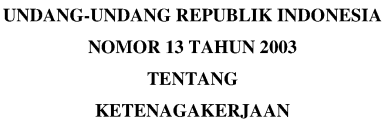
\includegraphics{pictures/pdf_example.png}
\caption{Gambar berkas PDF yang akan diekstraksi}
\end{figure}

akan dipindai menjadi

\begin{Shaded}
\begin{Highlighting}[]
\KeywordTok{-} \FunctionTok{xL:} \NormalTok{197.52}
  \FunctionTok{xR:} \NormalTok{442.79990000000004}
  \FunctionTok{'y':} \NormalTok{234.48000000000002}
  \FunctionTok{str:} \NormalTok{UNDANG-UNDANG REPUBLIK INDONESIA}
  \FunctionTok{pageNum:} \NormalTok{1}
  \FunctionTok{id:} \NormalTok{0}
\KeywordTok{-} \FunctionTok{xL:} \NormalTok{252.72}
  \FunctionTok{xR:} \NormalTok{387.6002}
  \FunctionTok{'y':} \NormalTok{255.12}
  \FunctionTok{str:} \NormalTok{NOMOR 13 TAHUN 2003}
  \FunctionTok{pageNum:} \NormalTok{1}
  \FunctionTok{id:} \NormalTok{1}
\KeywordTok{-} \FunctionTok{xL:} \NormalTok{291.12}
  \FunctionTok{xR:} \NormalTok{349.68048}
  \FunctionTok{'y':} \NormalTok{275.76}
  \FunctionTok{str:} \NormalTok{TENTANG}
  \FunctionTok{pageNum:} \NormalTok{1}
  \FunctionTok{id:} \NormalTok{2}
\KeywordTok{-} \FunctionTok{xL:} \NormalTok{257.28}
  \FunctionTok{xR:} \NormalTok{383.28015999999997}
  \FunctionTok{'y':} \NormalTok{296.4}
  \FunctionTok{str:} \NormalTok{KETENAGAKERJAAN}
  \FunctionTok{pageNum:} \NormalTok{1}
  \FunctionTok{id:} \NormalTok{3}
\end{Highlighting}
\end{Shaded}

\subsubsection{Membersihkan \emph{Noise} dari
Halaman}\label{membersihkan-noise-dari-halaman}

Tidak jarang dokumen peraturan Perudang-undangan mengandung data
\emph{noise} yang tidak ingin kita ekstraksi seperti \emph{header} dan
\emph{footer}. Pada penelitian ini, penulis menggunakan dokumen dari
sumber yang sama sehingga memiliki format yang sama, dan juga posisi
\emph{header} dan \emph{footer} yang hampir sama pada setiap dokumen.

\begin{figure}[htbp]
\centering

\includegraphics{pictures/pdf_header.png}
\caption{Contoh Header}
\end{figure}

Gambar diatas adalah contoh \emph{header} yang terdapat pada setiap
halaman. Dapat dilihat bahwa \emph{header} selalu terdiri dari teks
``PRESIDEN REPUBLIK INDONESIA'' dan diikuti oleh nomor halaman, dan
selalu terletak di posisi yang hampir sama. Oleh karena itu, penulis
memeriksa teks menggunakan \emph{regex} dan posisi dari setiap
\emph{span}, kemudian menghapus \emph{span} tersebut jika terdeteksi
sebagai header.

\subsubsection{Penggabungan Data Berkas PDF Asli dan Hasil OCR
Ulang}\label{penggabungan-data-berkas-pdf-asli-dan-hasil-ocr-ulang}

Pada proses ekstraksi berkas PDF menjadi daftar \emph{span}, penulis
menemukan satu masalah yaitu data hasil OCR tidak konsisten dalam
memindai angka. Seperti yang dapat dilihat pada gambar dibawah, angka 10
berhasil dipindai tetapi angka 9 tidak berhasil. Untuk kasus dibawah,
angka hanya tidak terpindai pada hasil OCR ulang, tetapi terpindai
dengan benar pada berkas PDF aslinya. Untuk menyelesaikan masalah
tersebut, penulis melakukan ekstraksi data pada berkas PDF aslinya,
kemudian menggabungkannya dengan data hasil pemindaian untuk melengkapi
bagian yang tidak terpindai.

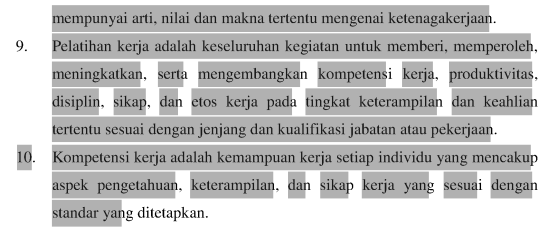
\includegraphics{pictures/pdf_unscanned_number.png})

Penulis hanya menggabungkan data dua berkas PDF untuk kasus angka
seperti yang disebutkan diatas. Hal tersebut dikarenakan pada umumnya
kita dapat mentolerir kesalahan pemindaian pada teks, tetapi karena
kegagalan pemindaian pada angka tersebut akan mempengaruhi struktur
dokumen, penulis memutuskan solusi diatas. Sebagai contoh, jika nomor 8
berhasil dipindai dan nomor 9 tidak berhasil, maka struktur akhir yang
dihasilkan akan mengandung semua isi nomor 9 didalam nomor 8, yang mana
seharusnya adalah nomor yang terpisah. Berikut berturut-turut adalah
contoh data yang dihasilkan jika nomor 9 tidak berhasil terpindai dan
jika berhasil terpindai.

Jika nomor 9 tidak berhasil terpindai:

\begin{Shaded}
\begin{Highlighting}[]
\KeywordTok{-} \FunctionTok{type:} \NormalTok{point}
  \FunctionTok{key:} \NormalTok{8}
  \FunctionTok{text:} \NormalTok{>-}
    \NormalTok{Informasi ketenagakerjaan adalah gabungan, rangkaian, dan analisis data yang}
    \NormalTok{berbentuk angka yang telah diolah, naskah dan dokumen yang mempunyai arti,}
    \NormalTok{nilai dan makna tertentu mengenai ketenagakerjaan.}
    \NormalTok{9. Pelatihan kerja adalah keseluruhan kegiatan untuk memberi, memperoleh,}
    \NormalTok{meningkatkan, serta mengembangkan kompetensi kerja, produktivitas, disiplin,}
    \NormalTok{sikap, dan etos kerja pada tingkat keterampilan dan keahlian tertentu sesuai}
    \NormalTok{dengan jenjang dan kualifikasi jabatan atau pekerjaan.}
\end{Highlighting}
\end{Shaded}

Jika nomor 9 berhasil terpindai:

\begin{Shaded}
\begin{Highlighting}[]
\KeywordTok{-} \FunctionTok{type:} \NormalTok{point}
  \FunctionTok{key:} \NormalTok{8}
  \FunctionTok{text:} \NormalTok{>-}
    \NormalTok{Informasi ketenagakerjaan adalah gabungan, rangkaian, dan analisis data yang}
    \NormalTok{berbentuk angka yang telah diolah, naskah dan dokumen yang mempunyai arti,}
    \NormalTok{nilai dan makna tertentu mengenai ketenagakerjaan.}
\KeywordTok{-} \FunctionTok{type:} \NormalTok{point}
  \FunctionTok{key:} \NormalTok{9}
  \FunctionTok{text:} \NormalTok{>-}
    \NormalTok{Pelatihan kerja adalah keseluruhan kegiatan untuk memberi, memperoleh,}
    \NormalTok{meningkatkan, serta mengembangkan kompetensi kerja, produktivitas, disiplin,}
    \NormalTok{sikap, dan etos kerja pada tingkat keterampilan dan keahlian tertentu sesuai}
    \NormalTok{dengan jenjang dan kualifikasi jabatan atau pekerjaan.}
\end{Highlighting}
\end{Shaded}

\subsection{Klasifikasi Dokumen}\label{klasifikasi-dokumen}

Pa

\subsection{Pengelompokan \emph{span} menjadi
Komponen}\label{pengelompokan-span-menjadi-komponen}

Teks yang membentuk suatu komponen terdiri dari satu atau lebih
\emph{span}, sehingga daftar \emph{span} yang didapatkan dari hasil
ekstraksi berkas PDF harus dikelompokkan sehingga setiap kelompok
merepresentasikan \emph{span} yang terdapat pada suatu komponen.
Pengelompokan dilakukan dengan mendeteksi \emph{span} awal dan
\emph{span} akhir dari sebuah komponen. Karena daftar \emph{span} hasil
ekstraksi bersifat 1 dimensi, hal ini bisa dilakukan dengan melakukan
iterasi pada setiap \emph{span}, kemudian menandai awal atau akhir dari
sebuah kelompok apabila memenuhi suatu pola. Setelah ditandai,
\emph{span} akan dikelompokkan sebagai daftar \emph{span} dari suatu
komponen.

Pengelompokan tidak langsund dilakukan dari daftar \emph{list} menjadi
daftar komponen, melainkan dibuat pengelompokan \emph{section} untuk
pembagian dokumen secara garis besar, kemudian baru dikelompokkan
sebagai komponen dari masing-masing \emph{section} tersebut. Pada gambar
dibawah \emph{section} ditandai dengan warna biru dan komponen ditandai
dengan warna merah. Dapat dilihat bahwa daftar \emph{span} data awal
dikelompokkan menjadi beberapa \emph{section} yaitu \texttt{judul},
\texttt{metadata}, \texttt{babset}, dan \texttt{disahkan}. Kemudian
\emph{span} pada section \texttt{babset} dikelompokkan menjadi komponen
bab yaitu \texttt{Bab 1}, \texttt{Bab 2}, dan \texttt{Bab 3}. Kemudian
\emph{span} pada setiap komponen bab dikelompokkan menjadi komponen
pasal. Pengelompokan bertingkat ini dilakukan agar fungsi untuk
mendeteksi batas antara komponen tidak menjadi rumit.

\begin{figure}[htbp]
\centering

\includegraphics{pictures/pdf_to_component.svg}
\caption{Ilustrasi Ekstraksi Daftar Span menjadi Data Struktur Komponen}
\end{figure}

Deteksi batas antara komponen atau \emph{section} dilakukan dengan
melihat data pada \emph{span} seperti \texttt{str}, \texttt{xL},
\texttt{xR}, dan \texttt{y}. Pada gambar diatas, pola yang terdeteksi
sebagai batas ditandai dengan huruf merah. Sebagai contoh, pada ekstraki
paling kiri, dari daftar \emph{span} asli menjadi \emph{section},
dilakukan iterasi \emph{span} dari atas dan akan dimasukkan ke dalam
\emph{section} \texttt{judul} sampai menemukan \emph{section} yang
diawali dengan kata \textbf{Menimbang}. Kemudian setiap \emph{span}
setelah span \textbf{Menimbang} tersebut akan dikelompokkan menjadi
\emph{section} \texttt{metadata} sampai menemukan section yang diawali
kata \textbf{BAB I}.

\subsubsection{Pengelompokan \emph{span} pada Komponen
Terurut}\label{pengelompokan-span-pada-komponen-terurut}

Beberapa komponen seperti \texttt{bab}, \texttt{bagian},
\texttt{paragraf}, \texttt{pasal}, \texttt{angka}, dan \texttt{huruf}
memiliki sifat terurut. Dalam hal ini, yang termasuk terurut adalah:

\begin{itemize}
\itemsep1pt\parskip0pt\parsep0pt
\item
  Komponen yang mengawali suatu komponen terurut akan selalu sama.
\item
  Hanya terdapat satu komponen yang dapat mengikuti komponen terurut.
\end{itemize}

Contoh dari sifat pertama adalah \texttt{bab}, \texttt{bagian},
\texttt{paragraf}, \texttt{pasal}, \texttt{angka} pasti dimulai dari
komponen nomor 1 seperti \texttt{bab 1} dan \texttt{pasal 1}, dan
\texttt{huruf} pasti dimulai dari komponen \texttt{huruf a}. Contoh dari
sifat kedua adalah hanya \texttt{pasal 2} yang dapat mengikuti
\texttt{pasal 1} dan hanya \texttt{huruf b} yang dapat mengikuti
\texttt{huruf a}. Dalam implementasi, penulis memastikan sifat-sifat ini
dipatuhi, sehingga sebagai contoh apabila sebuah dokumen terdeteksi
mengandung \texttt{bab 12} maka akan dijamin mengandung semua
\texttt{bab 1} sampai \texttt{bab 11} dan apabila terdeteksi mengandung
\texttt{pasal 196} maka akan dijamin mengandung semua pasal dari
\texttt{pasal 1} sampai \texttt{pasal 195}.

\subsubsection{Komponen Amandemen}\label{komponen-amandemen}

Mengekstraksi \emph{span} pada bagian amandemen merupakan salahsatu
tantangan pada penelitian ini. Dibawah adalah gambar amandemen pada
Pasal 17 UU Nomor 11 Tahun 2020 yang dilakukan terhadap Pasal 1 UU Nomor
26 Tahun 2007. Dapat dilihat bahwa kata \texttt{Pasal 17} dan
\texttt{Pasal 1} yang digunakan sebagai pembatas antara komponen
memiliki pola teks dan posisi yang hampir sama. Hal ini membuat
pembedaan antara ``Pasal biasa'' dan ``Pasal peng-amandemen'' menjadi
sulit dilakukan.

\begin{figure}[htbp]
\centering
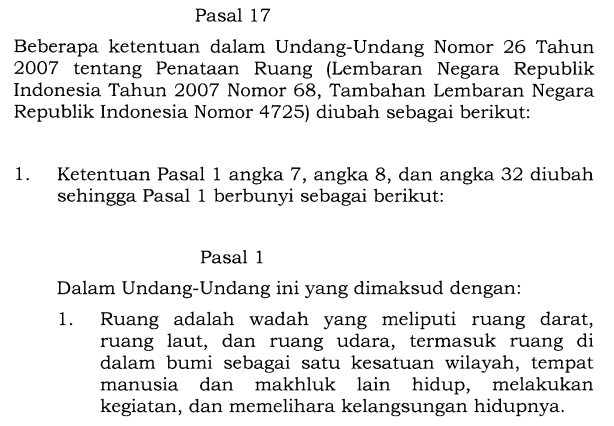
\includegraphics{pictures/pdf_amendment.png}
\caption{Contoh Amendemen pada UU Nomor 11 Tahun 2020}
\end{figure}

Untuk menyelesaikan masalah ini, penulis menggunakan koordinat
\texttt{xL} \emph{span} tepat setelah \emph{span} yang bertuliskan
``Pasal X''. Pada contoh deteksi kompoonen amandemen di bawah,
\texttt{xL} dari teks setelah pasal peng-amandemen (pasal biasa)
ditandai dengan lingkaran merah, \texttt{xL} dari pasal yang diamandemen
ditandai dengan lingkaran biru, dan garis hijau merepresentasikan batas
pemeda \texttt{xL} antara pasal biasa dan pasal yang diamandemen.
Pembedaan pasal biasa dan pasal amandemen hanya dilakukan jika dokumen
memiliki komponen berupa amandemen.

\begin{figure}[htbp]
\centering

\includegraphics{pictures/amendment_detection.svg}
\caption{Deteksi Komponen Amandemen}
\end{figure}

\subsection{Deteksi Sitasi}\label{deteksi-sitasi}

Setelah semua \emph{span} dikelompokan menjadi suatu komponen, dilakukan
deteksi sitasi pada teks pada setiap komponen untuk mengetahui apakah
komponen tersebut menyebut komponen atau dokumen peraturan
perundang-undangan lainnya. Berikut adalah daftar pola sitasi yang
berhasil dideteksi pada penelitian ini.

\begin{longtable}[c]{@{}lll@{}}
\toprule\addlinespace
Pola & Contoh teks & URI Terdeteksi
\\\addlinespace
\midrule\endhead
Undang Undang Dasar Negara Republik Indonesia Tahun 1945 & Undang Undang
Dasar Negara Republik Indonesia Tahun 1945 & /uud/
\\\addlinespace
Undang-Undang Nomor \{x\} Tahun \{y\} & Undang-Undang Nomor 26 Tahun
2007 & /uu/2007/26
\\\addlinespace
ayat (\{x\}) & ayat (1) & /uu/2003/13/pasal/169/ayat/1
\\\addlinespace
Pasal \{x\} & Pasal 156 & /uu/2003/13/pasal/156
\\\addlinespace
Pasal \{x\} ayat (\{y\}) & Pasal 156 ayat (2) &
/uu/2003/13/pasal/156/ayat/2
\\\addlinespace
huruf \{x\}, \{y\}, \ldots{} dan \{z\} & huruf a, b, c, d, dan e &
/uu/2003/13/menimbang/point/a
\\\addlinespace
& & /uu/2003/13/menimbang/point/b
\\\addlinespace
& & /uu/2003/13/menimbang/point/c
\\\addlinespace
& & /uu/2003/13/menimbang/point/d
\\\addlinespace
& & /uu/2003/13/menimbang/point/e
\\\addlinespace
huruf \{x\} dan \{y\} & huruf a dan b &
/uu/2003/13/pasal/1/point/5/point/a
\\\addlinespace
& & /uu/2003/13/pasal/1/point/5/point/b
\\\addlinespace
\bottomrule
\end{longtable}

Data sitasi mengandung data sebagai berikut:

\begin{itemize}
\itemsep1pt\parskip0pt\parsep0pt
\item
  \texttt{start}: \emph{index} karakter awal sitasi
\item
  \texttt{end}: \emph{index} karakter akhir sitasi
\item
  \texttt{uri}: URI dokumen dan
\end{itemize}

Berikut adalah contoh teks pada Undang-Undang Nomor 13 Tahun 2003 Pasal
158 Ayat (4) beserta sitasi yang terdeteksi.

\begin{Shaded}
\begin{Highlighting}[]
\FunctionTok{textString:} \NormalTok{>-}
  \NormalTok{Pekerja/buruh yang diputus hubungan kerjanya berdasarkan alasan sebagaimana}
  \NormalTok{dimaksud dalam ayat (1), dapat memperoleh uang penggantian hak sebagaimana}
  \NormalTok{dimaksud dalam Pasal 156 ayat (4).}
\FunctionTok{references:}
  \KeywordTok{-} \FunctionTok{start:} \NormalTok{91}
    \FunctionTok{end:} \NormalTok{99}
    \FunctionTok{uri:} \NormalTok{/uu/2003/13/pasal/158/ayat/1}
  \KeywordTok{-} \FunctionTok{start:} \NormalTok{166}
    \FunctionTok{end:} \NormalTok{184}
    \FunctionTok{uri:} \NormalTok{/uu/2003/13/pasal/156/ayat/4}
\end{Highlighting}
\end{Shaded}

Untuk melakukan deteksi, teks akan melalui fungsi yang masing-masing
memiliki pola untuk dideteksi. Oleh karena itu, untuk \emph{substring}
yang beririsan dapat memiliki lebih dari dua sitasi yang terdeteksi.
Pada kasus tersebut akan diambil sitasi dengan \emph{substring}
terpanjang. Sebagai contoh, teks ``Pasal 156 Ayat (4)'' pada UU No.13
Tahun 2003 Pasal 158 Ayat (4) akan terdeteksi sebagai 3 URI sitasi
sebagai berikut.

\begin{longtable}[c]{@{}ll@{}}
\toprule\addlinespace
Teks & URI
\\\addlinespace
\midrule\endhead
Pasal 156 Ayat (4) & \texttt{/uu/2003/13/pasal/156/ayat/4}
\\\addlinespace
Pasal 156 & \texttt{/uu/2003/13/pasal/156}
\\\addlinespace
Ayat (4) & \texttt{/uu/2003/13/pasal/158/ayat/4}
\\\addlinespace
\bottomrule
\end{longtable}

Pada kasus ini, yang akan diambil adalah teks ``Pasal 156 ayat (4)''
karena merupakan teks terpanjang.

\subsection{Data To MD}\label{data-to-md}

visualization

\subsection{Data to triple}\label{data-to-triple}

\subsubsection{triple definition}\label{triple-definition}

\subsubsection{triple to ttl}\label{triple-to-ttl}

\subsection{Query}\label{query}

Fuseki

\section{BAB 5 EVALUASI DAN ANALISIS
HASIL}\label{bab-5-evaluasi-dan-analisis-hasil}

\subsection{Aplikasi Knowledge Graph Peraturan
Perundang-undangan}\label{aplikasi-knowledge-graph-peraturan-perundang-undangan}

Dibuat \emph{chatbot} untuk mensimulasikan pengaplikasian KG.
\emph{Chatbot} akan memproses input yand diberikan oleh user, kemudian
meng-\emph{generate} SPARQL \emph{query}. Chatbot akan menampilkan hasil
dari \emph{query} tersebut.

\subsection{Evaluasi Hasil Konversi}\label{evaluasi-hasil-konversi}

Evaluasi akan dilakukan terhadap semua dokumen yang terdapat pada
peraturan.go.id. Selanjutnya dokumen-dokumen ini akan disebut dokument
tes.

\subsection{Evaluasi Manual}\label{evaluasi-manual}

Evaluasi kualitatif dilakukan terhadap sebagian dokumen yang didapatkan
dari hasil sam- pling dari dokumen tes. Seorang penilai akan melihat
markdown dari setiap dokumen hasil sampling, masing-masing dokumen akan
diberikan skor 0 sampai 100. Kualitas konversi dapat dilihat dari
rata-rata skor tersebut.

\subsection{Evaluasi Otomatis}\label{evaluasi-otomatis}

Evaluasi dilakukan dengan terlebih dahulu mendefinisikan metadata yang
pasti terdapat pada sebuah dokumen (misal, tempat dokumen disahkan),
kemudian menghitung sebera pa banyak metadata yang berhasil diekstrak.
Metadata hasil ekstraksi yang akan dihitung tidak perlu sesuai dengan
yang terdapat di dalam dokumen.

{[}6{]}:
\url{https://op.europa.eu/en/publication-detail/-/publication/514875b4-5efd-11e8-ab9c-01aa75ed71a}
1
